\chapter{Quotient Groups and Homomorphisms}

\section{Definitions and Examples}

Let $G$ and $H$ be groups.

\Exercise1 Let $\varphi\colon G\to H$ be a homomorphism and let $E$ be
a subgroup of $H$. Prove that $\varphi^{-1}(E)\leq G$ (i.e., the
preimage or pullback of a subgroup under a homomorphism is a
subgroup). If $E\trianglelefteq H$ prove that
$\varphi^{-1}(E)\trianglelefteq G$. Deduce that
$\ker\varphi\trianglelefteq G$.
\begin{proof}
  Note that $\varphi(1) = 1\in E$ so $\varphi^{-1}(E)$ is
  nonempty. Suppose $a, b \in \varphi^{-1}(E)$, so that
  $\varphi(a) = x$ and $\varphi(b) = y$ for some $x,y\in E$. Then,
  since $\varphi$ is a homomorphism, we have
  \begin{equation*}
    \varphi(ab^{-1}) = \varphi(a)\varphi(b)^{-1} = xy^{-1} \in E,
  \end{equation*}
  which shows that $ab^{-1}\in\varphi^{-1}(E)$. By the subgroup
  criterion, this shows that $\varphi^{-1}(E)\leq G$.

  Now suppose that $E$ is a normal subgroup of $H$. Let $g\in G$ and
  $n\in\varphi^{-1}(E)$. Then $\varphi(g) = h$ for some $h\in H$ and
  $\varphi(n) = x$ for some $x\in E$. We have
  \begin{align*}
    \varphi(gng^{-1})
    &= \varphi(g)\varphi(n)\varphi(g)^{-1} \\
    &= hxh^{-1}.
  \end{align*}
  But $hxh^{-1}\in E$ since $E\trianglelefteq H$, so
  $gng^{-1}\in\varphi^{-1}(E)$. The choice of $g$ and $n$ were
  arbitrary, so this shows that $\varphi^{-1}(E)\trianglelefteq G$.

  Lastly, if we let $E$ be the trivial subgroup of $H$, then the above
  shows that $\ker\varphi = \varphi^{-1}(E) \trianglelefteq G$ since
  the trivial subgroup is always normal.
\end{proof}

\Exercise2 Let $\varphi\colon G\to H$ be a homomorphism of groups with
kernel $K$ and let $a,b\in\varphi(G)$. Let $X\in G/K$ be the fiber
above $a$ and let $Y$ be the fiber above $b$, i.e.,
$X = \varphi^{-1}(a)$, $Y = \varphi^{-1}(b)$. Fix an element $u$ of
$X$ (so $\varphi(u) = a$). Prove that if $XY = Z$ in the quotient
group $G/K$ and $w$ is any member of $Z$, then there is some $v\in Y$
such that $uv = w$.
\begin{proof}
  Let $v = u^{-1}w$. We want to show that $v\in Y$, or
  $\varphi(v) = b$. Since $\varphi$ is a homomorphism and since
  $Z = \varphi^{-1}(ab)$, we have
  \begin{align*}
    \varphi(v) &= \varphi(u^{-1}w) \\
               &= \varphi(u)^{-1}\varphi(w) \\
               &= a^{-1}(ab) \\
               &= (a^{-1}a)b \\
               &= b.
  \end{align*}
  So $v\in Y$ as required.
\end{proof}

\Exercise3 Let $A$ be an abelian group and let $B$ be a subgroup of
$A$. Prove that $A/B$ is abelian. Give an example of a non-abelian
group $G$ containing a proper normal subgroup $N$ such that $G/N$ is
abelian.
\begin{solution}
  Let $a_1B, a_2B \in A/B$, where $a_1,a_2\in A$. Since $A$ is
  abelian, we have
  \begin{equation*}
    a_1Ba_2B = (a_1a_2)B = (a_2a_1)B = a_2Ba_1B.
  \end{equation*}
  Therefore $A/B$ is abelian.

  For the second part of the problem, let $G$ be the non-abelian
  dihedral group $D_8$ and let $N$ the proper normal subgroup
  $\gen{r^2}$. In the text it was shown that $G/N \cong V_4$, the
  Klein four-group, which is abelian. Therefore $G/N$ is abelian even
  though $G$ is not.
\end{solution}

\Exercise4
\label{exercise:quotient-group:coset-exponent}
Prove that in the quotient group $G/N$,
$(gN)^\alpha = g^\alpha N$ for all $\alpha\in\Z$.
\begin{proof}
  First, if $\alpha = 0$, then $(gN)^0 = 1N = g^0N$, so the statement
  is true in this case. We also know by Proposition~5 that
  $(gN)^{-1} = g^{-1}N$. So it will suffice to prove the statement
  only for positive $\alpha$, which we will do by induction on
  $\alpha$.

  The case where $\alpha = 1$ is trivial. For the inductive step,
  suppose that the statement $(gN)^k = g^kN$ holds for some particular
  $k\geq1$. Then
  \begin{align*}
    (gN)^{k+1}
    &= (gN)^kgN \\
    &= g^kNgN \\
    &= (g^kg)N \\
    &= g^{k+1}N.
  \end{align*}
  By induction, we conclude that $(gN)^\alpha = g^\alpha N$ for all
  $\alpha\geq1$, so the proof is complete.
\end{proof}

\Exercise5 Use the preceding exercise to prove that the order of the
element $gN$ in $G/N$ is $n$, where $n$ is the smallest positive
integer such that $g^n\in N$ (and $gN$ has infinite order if no such
positive integer exists). Give an example to show that the order of
$gN$ in $G/N$ may be strictly smaller than the order of $g$ in $G$.
\begin{solution}
  Fix an element $gN$ in $G/N$. First, if possible, let $n$ be the
  smallest positive integer such that $g^n\in N$. Then $g^nN =
  1N$. So, by the previous exercise, we know that $(gN)^n = 1N$. This
  shows that $\ord{gN}\leq n$. On the other hand, if $m$ is any
  positive integer with $(gN)^m = 1N$ then, using the previous
  exercise again, $g^mN = 1N$ so that $g^m\in N$. Since $n$ is the
  smallest positive integer with $g^n\in N$, this shows that
  $\ord{gN}\geq n$, which completes the proof for the case of finite
  order.

  Next, suppose that there is no such $n$. Then for each positive
  integer $k$, $g^k\not\in N$. If $gN$ were to have finite order, say
  $(gN)^m = 1N$, then the previous exercise would show that
  $g^m\in N$, giving a contradiction. This shows that $gN$ has
  infinite order, which completes the proof.

  Lastly, for the example, consider $G = Z_4$, the cyclic group of
  order $4$. Let $x$ be a generator for $G$ and take
  $N = \gen{x^2} = \{1, x^2\}$. Now the element $x^2$ has order $2$ in
  $G$, but $x^2N = 1N$ has order $1$ in $G/N$.
\end{solution}

\Exercise6 Define $\varphi\colon\R^\times\to\{\pm1\}$ by letting
$\varphi(x)$ be $x$ divided by the absolute value of $x$. Describe the
fibers of $\varphi$ and prove that $\varphi$ is a homomorphism.
\begin{solution}
  The fiber above $1$ is the positive reals, and the fiber above $-1$
  is the negative reals.

  Let $x,y\in\R^\times$ be arbitrary. Then
  \begin{equation*}
    \varphi(xy)
    = \frac{xy}{\abs{xy}}
    = \frac{x}{\abs{x}}\cdot\frac{y}{\abs{y}}
    = \varphi(x)\varphi(y),
  \end{equation*}
  so $\varphi$ is a homomorphism.
\end{solution}

\Exercise7 Define $\pi\colon\R^2\to\R$ by $\pi((x,y)) = x + y$. Prove
that $\pi$ is a surjective homomorphism and describe the kernel and
fibers of $\pi$ geometrically.
\begin{solution}
  For any $(x_1,y_1), (x_2,y_2)\in\R^2$, we have
  \begin{align*}
    \pi((x_1,y_1) + (x_2,y_2))
    &= \pi((x_1 + x_2, y_1 + y_2)) \\
    &= (x_1 + x_2) + (y_1 + y_2) \\
    &= (x_1 + y_1) + (x_2 + y_2) \\
    &= \pi((x_1,y_1)) + \pi((x_2,y_2)),
  \end{align*}
  so $\pi$ is a homomorphism. And for any $x\in\R$, we have
  $\pi((x, 0)) = x + 0 = x$, so $\pi$ is also surjective.

  $\ker\pi$ is simply the diagonal line whose equation is $x + y =
  0$. And for $a\in\R$, the fiber over $a$ is the line with equation
  $x + y = a$, which is just a translate of the kernel.
\end{solution}

\Exercise8 Let $\varphi\colon\R^\times\to\R^\times$ be the map sending
$x$ to the absolute value of $x$. Prove that $\varphi$ is a
homomorphism and find the image of $\varphi$. Describe the kernel and
the fibers of $\varphi$.
\begin{solution}
  For any $x,y\in\R^\times$ we have
  \begin{equation*}
    \varphi(xy) = \abs{xy} = \abs{x}\abs{y} = \varphi(x)\varphi(y)
  \end{equation*}
  and $\varphi$ is a homomorphism. Its image is $\R^+$, the positive
  reals.

  The kernel of $\varphi$ is the set $\{-1,1\}$, since
  $\varphi(\pm1) = 1$ and no other real number has an absolute value
  of $1$. Likewise, the fiber over the real number $a$ is $\{-a, a\}$.
\end{solution}

\Exercise9 Define $\varphi\colon\C^\times\to\R^\times$ by
$\varphi(a + bi) = a^2 + b^2$. Prove that $\varphi$ is a homomorphism
and find the image of $\varphi$. Describe the kernel and the fibers of
$\varphi$ geometrically (as subsets of the plane).
\begin{solution}
  Let $a + bi$ and $c + di$ be any members of $\C^\times$. Then
  \begin{align*}
    \varphi((a + bi)(c + di))
    &= \varphi((ac - bd) + (ad + bc)i) \\
    &= (ac - bd)^2 + (ad + bc)^2 \\
    &= a^2c^2 - 2abcd + b^2d^2 + a^2d^2 + 2abcd + b^2c^2 \\
    &= a^2(c^2 + d^2) + b^2(c^2 + d^2) \\
    &= (a^2 + b^2)(c^2 + d^2) \\
    &= \varphi(a + bi)\varphi(c + di),
  \end{align*}
  and $\varphi$ is a homomorphism. Let $a+bi\in\C^\times$. Since $a$
  and $b$ cannot both be zero, $a^2 + b^2 > 0$. So
  $\im\varphi\subseteq\R^+$. But for any $a\in\R^+$, we have
  $\varphi(\sqrt{a} + 0i) = a$ and we see that $\im\varphi = \R^+$.

  The kernel of $\varphi$ is the set
  \begin{equation*}
    \ker\varphi = \{a + bi\in\C^\times \mid a^2 + b^2 = 1\}.
  \end{equation*}
  This is a circle of radius 1 centered at the origin in the complex
  plane. For $a\in\R^+$, the fiber over $a$ is the circle of radius
  $\sqrt{a}$.
\end{solution}

\Exercise{10} Let $\varphi\colon\Z/8\Z\to\Z/4\Z$ by
$\varphi(\bar a) = \bar a$. Show that this is a well defined,
surjective homomorphism and describe its fibers and kernel explicitly
(showing that $\varphi$ is well defined involves the fact that
$\bar a$ has a different meaning in the domain and range of
$\varphi$).
\begin{solution}
  To show that $\varphi$ is well defined we need to show that any
  choice of representative for a particular congruence class in
  $\Z/8\Z$ will produce the same congruence class in $\Z/4\Z$ under
  $\varphi$. Suppose then that $\bar a = \bar b$, where
  $\bar a,\bar b\in\Z/8\Z$. Then for some integer $k$, $a = b + 8k$
  and we have
  \begin{align*}
    \varphi(\bar a)
    &= \varphi(\overline{b + 8k}) \\
    &= \overline{b + 8k} \\
    &= \overline{b + 4(2k)} \\
    &= \bar b \\
    &= \varphi(\bar b)
  \end{align*}
  and $\varphi$ is well defined. It is also a homomorphism since
  \begin{align*}
    \varphi(\bar a + \bar b)
    &= \varphi(\overline{a + b}) \\
    &= \overline{a + b} \\
    &= \bar a + \bar b \\
    &= \varphi(\bar a) + \varphi(\bar b).
  \end{align*}
  And it is clearly surjective.

  The fibers of $\varphi$ are
  \begin{align*}
    \varphi^{-1}(\bar0) &= \{\bar0, \bar4\}, \\
    \varphi^{-1}(\bar1) &= \{\bar1, \bar5\}, \\
    \varphi^{-1}(\bar2) &= \{\bar2, \bar6\}, \\
    \varphi^{-1}(\bar3) &= \{\bar3, \bar7\},
  \end{align*}
  and $\ker\varphi = \varphi^{-1}(\bar0) = \{\bar0, \bar4\}$.
\end{solution}

\Exercise{11} Let $F$ be a field and let
\begin{equation*}
  G = \left\{
    \begin{pmatrix}
      a & b \\
      0 & c
    \end{pmatrix}
    \;\;\middle|\;\;
    a,b,c\in F,\;\; ac\neq0
  \right\}
  \leq GL_2(F).
\end{equation*}
\begin{enumerate}
\item Prove that the map
  \begin{equation*}
    \varphi\colon
    \begin{pmatrix}
      a & b \\ 0 & c
    \end{pmatrix}
    \mapsto a
  \end{equation*}
  is a surjective homomorphism from $G$ onto $F^\times$. Describe the
  fibers and kernel of $\varphi$.
  \begin{solution}
    First, for any $a\in F^\times$, we have
    \begin{equation*}
      \varphi\left(
      \begin{pmatrix}
        a & 1 \\ 0 & 1
      \end{pmatrix}
      \right) = a,
    \end{equation*}
    so $\varphi$ is surjective. And for any $a,b,c,d,e,f\in F$ with
    $ac\neq0$ and $df\neq0$, we have
    \begin{align*}
      \varphi\left(\begin{pmatrix} a & b \\ 0 & c \end{pmatrix}
              \begin{pmatrix} d & e \\ 0 & f \end{pmatrix}\right)
      &= \varphi\left(\begin{pmatrix} ad & ae + bf \\
          0 & cf \end{pmatrix}\right) \\
      &= ad \\
      &= \varphi\left(\begin{pmatrix} a & b \\ 0 & c \end{pmatrix}\right)
         \varphi\left(\begin{pmatrix} d & e \\ 0 & f \end{pmatrix}\right),
    \end{align*}
    so $\varphi$ is a homomorphism.

    For each $a\in F^\times$, the fiber over $a$ is given by
    \begin{equation*}
      \varphi^{-1}(a) =
      \left\{
        \begin{pmatrix}
          a & x \\
          0 & y
        \end{pmatrix}
        \;\;\middle|\;\;
        x,y\in F,\;\;y\neq0
      \right\},
    \end{equation*}
    with the kernel being the fiber above $1$.
  \end{solution}

\item Prove that the map
  \begin{equation*}
    \psi\colon
    \begin{pmatrix}
      a & b \\ 0 & c
    \end{pmatrix}
    \mapsto (a,c)
  \end{equation*}
  is a surjective homomorphism from $G$ onto
  $F^\times\times F^\times$. Describe the fibers and kernel of $\psi$.
  \begin{solution}
    The proof is entirely similar to the proof for $\varphi$ in the
    previous part of the problem and is omitted here. The fiber over
    $(a,c)$ is
    \begin{equation*}
      \psi^{-1}((a,c)) =
      \left\{
        \begin{pmatrix}
          a & x \\
          0 & c
        \end{pmatrix}
        \;\;\middle|\;\;
        x\in F
      \right\},
    \end{equation*}
    with $\ker\psi = \psi^{-1}((1,1))$.
  \end{solution}

\item Let
  \begin{equation*}
    H = \left\{
      \begin{pmatrix}
        1 & b \\ 0 & 1
      \end{pmatrix}
      \;\middle|\;
      b\in F
    \right\}.
  \end{equation*}
  Prove that $H$ is isomorphic to the additive group $F$.
  \begin{proof}
    Define $\rho\colon H\to F$ by
    \begin{equation*}
      \rho\left(
        \begin{pmatrix}
          1 & b \\
          0 & 1
        \end{pmatrix}
      \right) = b.
    \end{equation*}
    Then $\rho$ is a bijection since it has the obvious two-sided
    inverse $\rho^{-1}\colon F\to H$ given by
    \begin{equation*}
      \rho^{-1}(b) =
      \begin{pmatrix}
        1 & b \\
        0 & 1
      \end{pmatrix},
    \end{equation*}
    and it is a homomorphism since
    \begin{align*}
      \rho\left(
      \begin{pmatrix}
        1 & b_1 \\ 0 & 1
      \end{pmatrix}
      \begin{pmatrix}
        1 & b_2 \\ 0 & 1
      \end{pmatrix}
      \right)
      &= \rho\left(
        \begin{pmatrix}
          1 & b_1 + b_2 \\ 0 & 1
        \end{pmatrix}
      \right) \\
      &= b_1 + b_2 \\
      &= \rho\left(
      \begin{pmatrix}
        1 & b_1 \\ 0 & 1
      \end{pmatrix}\right) +
      \rho\left(\begin{pmatrix}
        1 & b_2 \\ 0 & 1
      \end{pmatrix}
      \right).
    \end{align*}
    Therefore $\rho$ is an isomorphism and $H\cong F$.
  \end{proof}
\end{enumerate}

\Exercise{12}
\label{exercise:quotient-group:r-to-s1-kernel}
Let $G$ be the additive group of real numbers, let $H$
be the multiplicative group of complex numbers of absolute value $1$
(the unit circle $S^1$ in the complex plane) and let
$\varphi\colon G\to H$ be the homomorphism
$\varphi\colon r\mapsto e^{2\pi ir}$. Draw the points on a real line
which lie in the kernel of $\varphi$. Describe similarly the elements
in the fibers of $\varphi$ above the points $-1$, $i$, and
$e^{4\pi i/3}$ of $H$.
\begin{solution}
  The kernel of $\varphi$ is simply $\Z$, since $e^{2\pi ir} = 1$ if
  and only if $r$ is an integer:
  \begin{center}
    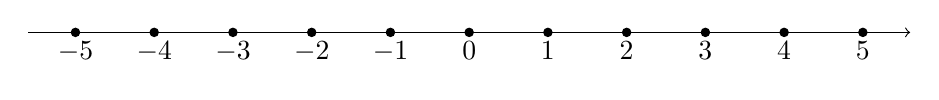
\begin{tikzpicture}
      \draw [->] (-5.6,0) -- (5.6,0);
      \foreach \i in {-5,...,5}{
        \draw [fill] (\i,0) circle [radius=1.5pt];
        \node [below] at (\i,0) {$\i$};
      }
    \end{tikzpicture}
  \end{center}

  The specified fibers are
  \begin{align*}
    \varphi^{-1}(-1)
    &= \frac12 + \Z = \left\{k + \frac12 \;\middle|\; k\in\Z\right\}, \\
    \varphi^{-1}(i)
    &= \frac14 + \Z = \left\{k + \frac14 \;\middle|\; k\in\Z\right\}, \\
    \varphi^{-1}(e^{4\pi i/3})
    &= \frac23 + \Z = \left\{k + \frac23 \;\middle|\; k\in\Z\right\}.
      \qedhere
  \end{align*}
\end{solution}

\Exercise{13} Repeat the preceding exercise with the map $\varphi$
replaced by the map $\varphi\colon r\mapsto e^{4\pi ir}$.
\begin{solution}
  In this case the kernel is $\frac12\Z$:
  \begin{center}
    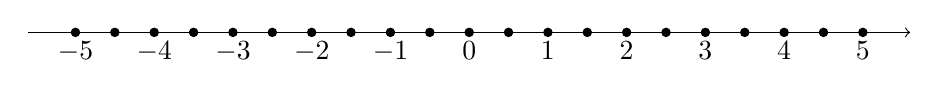
\begin{tikzpicture}
      \draw [->] (-5.6,0) -- (5.6,0);
      \foreach \i in {-5,...,5}{
        \draw [fill] (\i,0) circle [radius=1.5pt];
        \node [below] at (\i,0) {$\i$};
      }
      \foreach \i in {-5,...,4}{
        \draw [fill] (\i + 1/2,0) circle [radius=1.5pt];
      }
    \end{tikzpicture}
  \end{center}

  The fibers are
  \begin{align*}
    \varphi^{-1}(-1)
    &= \frac14 + \frac12\Z
      = \left\{\frac{2k+1}4 \;\middle|\; k\in\Z\right\}, \\
    \varphi^{-1}(i)
    &= \frac18 + \frac12\Z
      = \left\{\frac{4k+1}8 \;\middle|\; k\in\Z\right\}, \\
    \varphi^{-1}(e^{4\pi i/3})
    &= \frac13 + \frac12\Z
      = \left\{\frac{3k+2}6 \;\middle|\; k\in\Z\right\}.
      \qedhere
  \end{align*}
\end{solution}

\Exercise{14} Consider the additive quotient group $\Q/\Z$.
\begin{enumerate}
\item Show that every coset of $\Z$ in $\Q$ contains exactly one
  representative $q\in\Q$ in the range $0\leq q<1$.
  \begin{proof}
    Let $t\in\Q$ be arbitrary. Write $t = m/n$ in lowest terms. We may
    use the division algorithm to find unique integers $q$ and $r$
    with $0\leq r<n$ such that $m = nq + r$. Then $t = q + r/n$, where
    $0\leq r/n<1$. Then we have
    \begin{equation*}
      t + \Z = \{t + k\mid k\in\Z\}
      = \left\{\frac{r}n + (k+q) \;\middle|\; k\in\Z\right\}
      = \frac{r}n + \Z.
    \end{equation*}
    From the uniqueness of $q$ and $r$, it follows that $r/n$ is the
    only representative of $t + \Z$ that is in the range $[0,1)$.
  \end{proof}
\item Show that every element of $\Q/\Z$ has finite order but that
  there are elements of arbitrarily large order.
  \begin{proof}
    Again, let $t\in\Q$ be arbitrary, with $t = m/n$ for integers $m$
    and $n$, with $n>0$. Then
    \begin{equation*}
      n(t + \Z) = nt + \Z = m + \Z = 0 + \Z,
    \end{equation*}
    so $t + \Z$ has finite order (note that the first equality follows
    from Exercise~\ref{exercise:quotient-group:coset-exponent}).

    Given any positive integer $k$, the coset $1/k + \Z$ has order
    $k$. Since $k$ can be made arbitrarily large, we see that $\Q/\Z$
    contains elements of arbitrarily large order.
  \end{proof}
\item Show that $\Q/\Z$ is the torsion subgroup of $\R/\Z$.
  \begin{proof}
    We need to show that the only elements in $\R/\Z$ having finite
    order belong to $\Q/\Z$. So suppose $r$ is an irrational
    representative of a coset having finite order $n$. Then
    \begin{equation*}
      nr + \Z = n(r + \Z) = 0 + \Z.
    \end{equation*}
    This implies that $nr\in\Z$, say $m = nr$. Then $r = m/n$ and
    $r\in\Q$, contradicting our choice of $r$. Therefore $r$ cannot
    have finite order. So $\Q/\Z$ is indeed the torsion subgroup of
    $\R/\Z$.
  \end{proof}
\item Prove that $\Q/\Z$ is isomorphic to the multiplicative group of
  roots of unity in $\C^\times$.
  \begin{proof}
    Let $S^1$ be the unit circle in the complex plane and let $G$ be
    the multiplicative group of the roots of unity. From
    Exercise~\ref{exercise:quotient-group:r-to-s1-kernel} we know that
    $\R/\Z \cong S^1$, as we can exhibit the explicit isomorphism
    $\varphi$ by
    \begin{equation*}
      \varphi(r + \Z) = e^{2\pi ir}.
    \end{equation*}

    Now consider the torsion subgroup of $S^1$. By definition, $z\in S^1$
    has finite order, say $n$, if and only if $z^n = 1$, i.e. if and
    only if $z\in G$. So we see that $G$ is actually the torsion
    subgroup of $S^1$.

    Since $\R/\Z$ is isomorphic to $S^1$, it follows that their
    torsion subgroups are also isomorphic. Hence $\Q/\Z\cong G$.
  \end{proof}
\end{enumerate}
